\section{Experimentos e resultados}


\subsection{Experimentos}
Isso \'e o exemplo do experimento 1.
Ele consiste em analizar o tempo de converg\^encia entre a mudan\c{c}a de comunica\c{c}\~ao de n\'os entre o Soldado 2 e o Soldado 4.
\begin{figure}[htb]
	\centering
	\includegraphics[scale=0.5]{experimento1.eps}
	\caption{Experimento 1}
	\label{figExp1}
\end{figure}

\begin{figure}[htb]
	\centering
	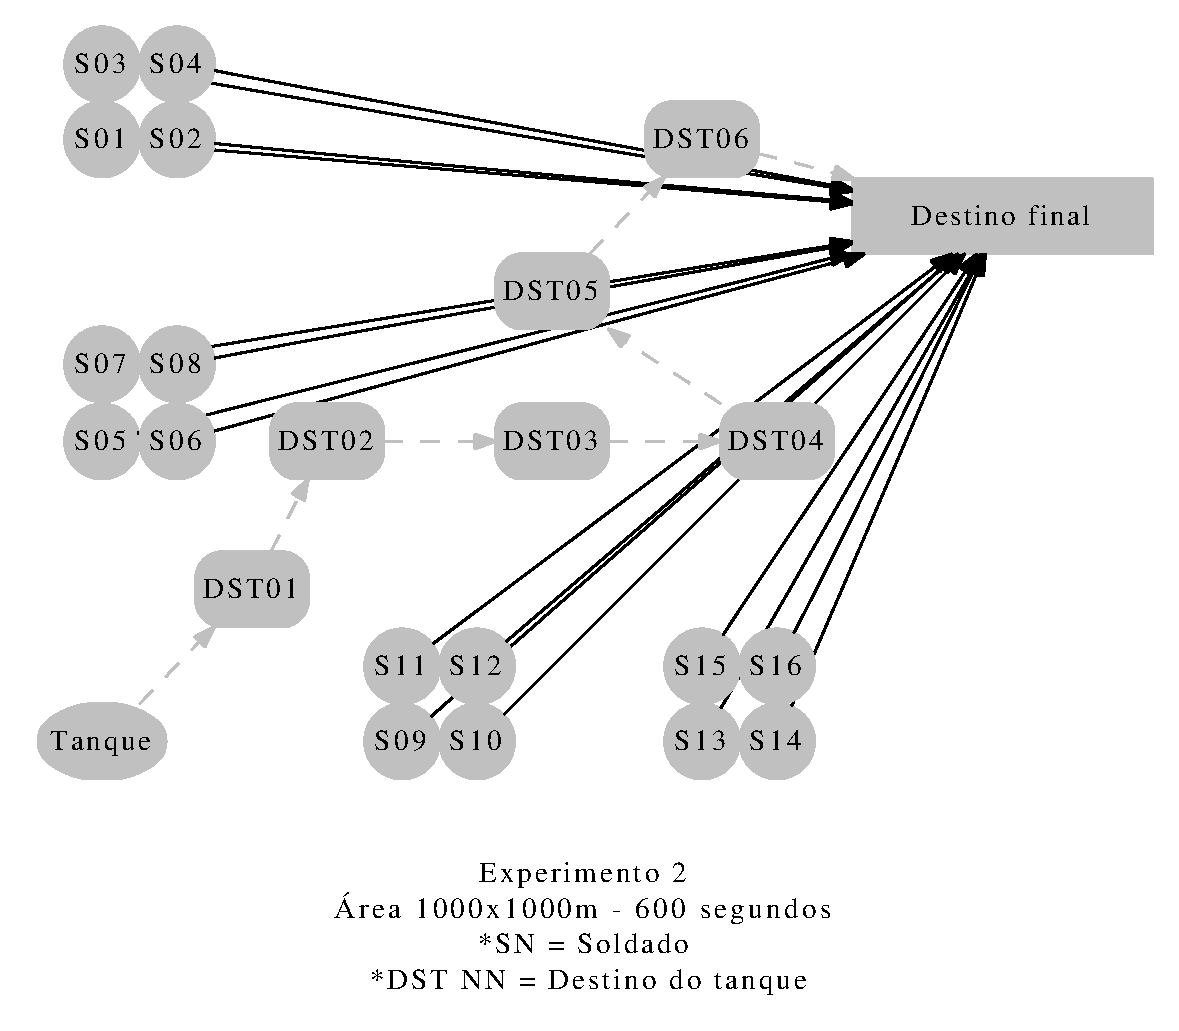
\includegraphics[scale=0.5]{experimento2.eps}
	\caption{Experimento 2}
	\label{figExp2}
\end{figure}


\subsection{M\'etricas}
As seguintes m\'etricas foram utilizadas:


\subsection{An\'alise comparativa dos resultados}


